\documentclass{article}
\usepackage{graphicx}
\usepackage{verbatim}
\usepackage{hyperref}
%\usepackage[T1]{fontenc}
%\renewcommand*\familydefault{\sfdefault}
%\usepackage{times}
\graphicspath{ {./images} }
\counterwithin{figure}{section}

\title{Report for Image Processing Assessment}
\author{Timothy Smith \\
        Email: \href{mailto:25796944@students.lincoln.ac.uk}{25796944@students.lincoln.ac.uk} \\
        Student ID: 25796944}

\begin{document}
\begin{titlepage}
\maketitle

\end{titlepage}

\section{Pre-processing}
\subsection{Grayscale Conversion}
The first step of the process is grayscale conversion.
For the purposes of shape based object detection, colour is often a
variable that only complicates processing and can be removed to
simplify the process.

The code for grayscale
conversion is already provided in \texttt{Task1to4.m} as
given which uses the 
built-in function \texttt{rbg2gray}.

\subsection{Size Reduction}
Reducing the size of an image can be an excellent way to improve
the performace of an object detection algorithm, by simply reducing
the amount of data required to be processed. This has to be done
within reason, of course, since reducing the image
too far will cause of loss of information. Here to produce the image
shown in figure \ref{fig:scaled}
the built in function
\texttt{imresize} is used. The image is scaled by half using bilinear
interpolation as required using the code below:
\begin{verbatim}
I_scaled = imresize(I_gray, 0.5, 'bilinear');
\end{verbatim}

\begin{figure}[hbt!]
\begin{center}
\begin{minipage}{0.4\textwidth}
	\caption{Image after scaling}
	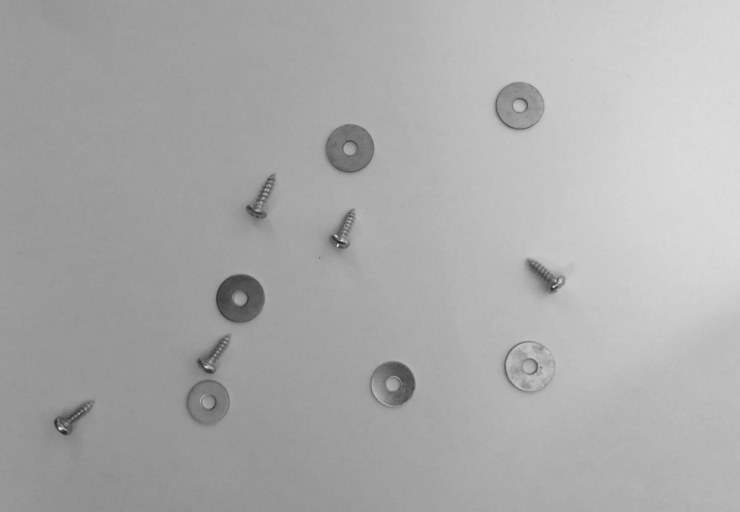
\includegraphics[width=\textwidth]{scaled}
	\label{fig:scaled}
\end{minipage}
\end{center}
\end{figure}

\subsection{Enhancement}
Note to self: this is subject to improvement.

In order to enhance the image we use the built-in function 
\texttt{imadjust}. This consists of simply passing the scaled image
as an argument:

\begin{verbatim}
I_adjusted = imadjust(I_scaled);
\end{verbatim}

\begin{figure}[hbt!]
\begin{minipage}{0.3\textwidth}
	\caption{Histogram prior to enhancement}
	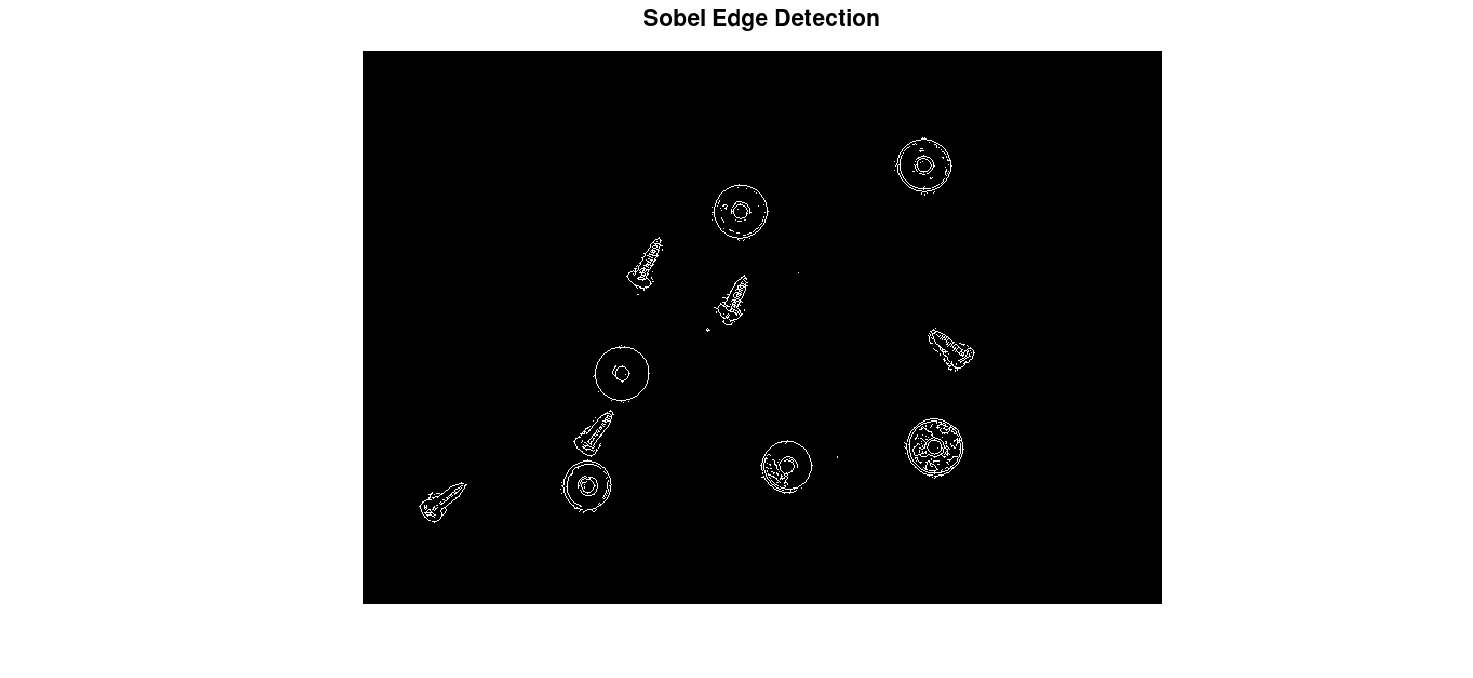
\includegraphics[width=\textwidth]{scaled_histogram}
	\label{fig:scaled_histogram}
\end{minipage}
\begin{minipage}{0.3\textwidth}
	\caption{Histogram after enhancement}
	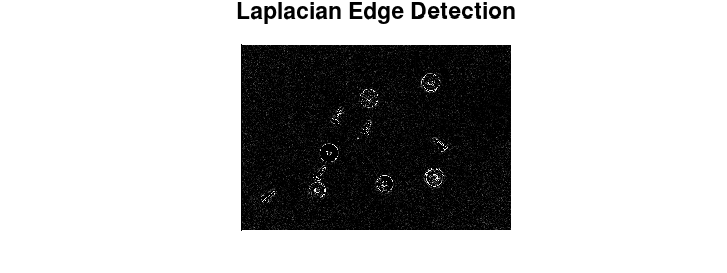
\includegraphics[width=\textwidth]{enhanced_histogram}
	\label{fig:enhanced_histogram}
\end{minipage}
\begin{minipage}{0.3\textwidth}
	\caption{Image after enhancement}
	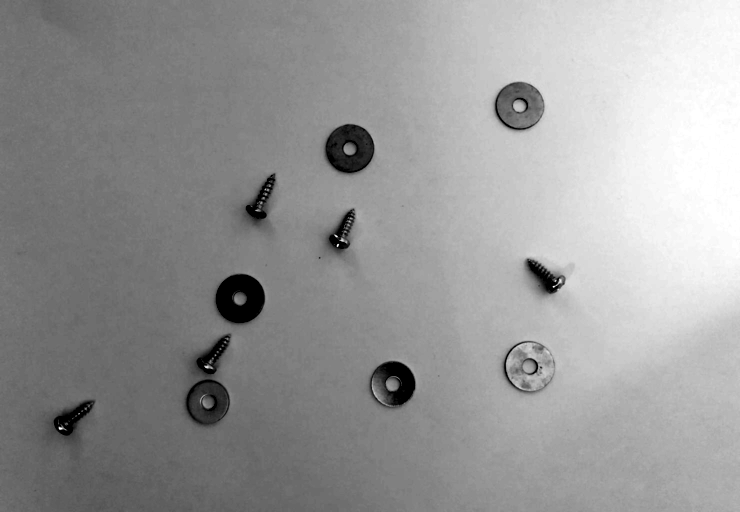
\includegraphics[width=\textwidth]{enhanced}
	\label{fig:enhanced}
\end{minipage}
\end{figure}

\subsection{Binarisation}
To binarise the image we call the built in function
\texttt{im2bw}:

\begin{verbatim}
I_binarised = imadjust(I_enhanced); <<< FIX
\end{verbatim}

blah blah splitting blah blah XXX binarisation.

\section{Edge Detection}
My approach here was to try a variety of edge detection methods and;
see which one produced the most promising results.

The best looking turned out to be Canny, likely because XXX.

\section{Simple Segmentation}


We XXX the image to reduce noise and artefacts.

\section{Object Recognition}
Advantage is taken of the XXX method and we consider the circularity
(I think that's the word) of the various objects.
\section{Robust Method}
Since we are required to avoid manually creating thresholds as much
as possible, binarisation does not seem to be a robust segmentation
method. This isn't an issue better enhancement either, since some
of the washers and screws are lighter in the images than some of the
background thanks to the unfavourable lighting conditions.

To devise a method that works more widely we need to return to
edge detection methods applied to the enhanced (not binarised)
image.

\section{Performance Evaluation}
\section*{Appendix}
\subsection*{Task1to4.m}
\verbatiminput{../code/Task1to4.m}
\subsection*{Task5to6.m}
\verbatiminput{../code/Task5to6.m}

\end{document}
